%%
%% This is file `sample-manuscript.tex',
%% generated with the docstrip utility.
%%
%% The original source files were:
%%
%% samples.dtx  (with options: `manuscript')
%% 
%% IMPORTANT NOTICE:
%% 
%% For the copyright see the source file.
%% 
%% Any modified versions of this file must be renamed
%% with new filenames distinct from sample-manuscript.tex.
%% 
%% For distribution of the original source see the terms
%% for copying and modification in the file samples.dtx.
%% 
%% This generated file may be distributed as long as the
%% original source files, as listed above, are part of the
%% same distribution. (The sources need not necessarily be
%% in the same archive or directory.)
%%
%%
%% Commands for TeXCount
%TC:macro \cite [option:text,text]
%TC:macro \citep [option:text,text]
%TC:macro \citet [option:text,text]
%TC:envir table 0 1
%TC:envir table* 0 1
%TC:envir tabular [ignore] word
%TC:envir displaymath 0 word
%TC:envir math 0 word
%TC:envir comment 0 0
%%
%%
%% The first command in your LaTeX source must be the \documentclass command.
\documentclass[manuscript,screen,review]{acmart}

%%
%% \BibTeX command to typeset BibTeX logo in the docs
\AtBeginDocument{%
  \providecommand\BibTeX{{%
    Bib\TeX}}}

%% Rights management information.  This information is sent to you
%% when you complete the rights form.  These commands have SAMPLE
%% values in them; it is your responsibility as an author to replace
%% the commands and values with those provided to you when you
%% complete the rights form.
\setcopyright{acmcopyright}
\copyrightyear{2018}
\acmYear{2018}
\acmDOI{XXXXXXX.XXXXXXX}

%% These commands are for a PROCEEDINGS abstract or paper.
\acmConference[Conference acronym 'XX]{Make sure to enter the correct
  conference title from your rights confirmation emai}{June 03--05,
  2018}{Woodstock, NY}
\acmPrice{15.00}
\acmISBN{978-1-4503-XXXX-X/18/06}


%%
%% Submission ID.
%% Use this when submitting an article to a sponsored event. You'll
%% receive a unique submission ID from the organizers
%% of the event, and this ID should be used as the parameter to this command.
%%\acmSubmissionID{123-A56-BU3}

%%
%% For managing citations, it is recommended to use bibliography
%% files in BibTeX format.
%%
%% You can then either use BibTeX with the ACM-Reference-Format style,
%% or BibLaTeX with the acmnumeric or acmauthoryear sytles, that include
%% support for advanced citation of software artefact from the
%% biblatex-software package, also separately available on CTAN.
%%
%% Look at the sample-*-biblatex.tex files for templates showcasing
%% the biblatex styles.
%%

%%
%% The majority of ACM publications use numbered citations and
%% references.  The command \citestyle{authoryear} switches to the
%% "author year" style.
%%
%% If you are preparing content for an event
%% sponsored by ACM SIGGRAPH, you must use the "author year" style of
%% citations and references.
%% Uncommenting
%% the next command will enable that style.
%%\citestyle{acmauthoryear}

\author{Alex Groce}
\affiliation{\institution{Northern Arizona University}\country{United States}}

\author{Kush Jain}
\affiliation{\institution{Carnegie Mellon University}\country{United States}}

\author{Goutamkumar Tulajappa Kalburgi}
\affiliation{\institution{Northern Arizona University}\country{United States}}

\author{Claire Le Goues}
\affiliation{\institution{Carnegie Mellon University}\country{United States}}

\author{Rahul Gopinath}
\affiliation{\institution{University of Sydney}\country{Australia}}

\usepackage{code}
\usepackage{url}

%%
%% By default, the full list of authors will be used in the page
%% headers. Often, this list is too long, and will overlap
%% other information printed in the page headers. This command allows
%% the author to define a more concise list
%% of authors' names for this purpose.
\renewcommand{\shortauthors}{Alex Groce, Kush Jain, Rijnard van Tonder, Goutamkumar Tulajappa Kalburgi, Claire Le Goues}

%%
%% end of the preamble, start of the body of the document source.
\begin{document}

%%
%% The "title" command has an optional parameter,
%% allowing the author to define a "short title" to be used in page headers.
\title{Registered Report: First, Fuzz the Mutants}

%%
%% The "author" command and its associated commands are used to define
%% the authors and their affiliations.
%% Of note is the shared affiliation of the first two authors, and the
%% "authornote" and "authornotemark" commands
%% used to denote shared contribution to the research.

%%
%% By default, the full list of authors will be used in the page
%% headers. Often, this list is too long, and will overlap
%% other information printed in the page headers. This command allows
%% the author to define a more concise list
%% of authors' names for this purpose.
\renewcommand{\shortauthors}{Groce et al.}

%%
%% The abstract is a short summary of the work to be presented in the
%% article.
\begin{abstract}
Most fuzzing efforts, very understandably, focus on fuzzing the program
in which bugs are to be found.  However, in this paper we propose that
fuzzing programs ``near'' the System Under Test (SUT) can in fact
improve the effectiveness of fuzzing, even if it means less time is
spent fuzzing the actual target system.  In particular, we claim that
fault detection and code coverage can be improved by splitting fuzzing
resources between the SUT and \emph{mutants} of the SUT.  Spending
half of a fuzzing budget fuzzing mutants, and then using the seeds
generated to fuzz the SUT can allow a fuzzer to explore more behaviors
than spending the entire fuzzing budget on the SUT.  The approach
works because fuzzing most mutants is ``almost'' fuzzing the SUT, but
may change behavior in ways that allow a fuzzer to reach deeper
program behaviors.  Our results using Google's FuzzBench platform show that fuzzing mutants
is trivial to implement and fuzzer-agnostic, but provides clear, statistically significant
benefits in terms of branch coverage for a number of
real-world benchmarks, using AFLplusplus and Honggfuzz as baseline
fuzzers.  One of the variants of our method, using heuristically
chosen mutants,  ranks first by both of the two standard measures of fuzzer effectiveness
provided by FuzzBench.
\end{abstract}

%%
%% The code below is generated by the tool at http://dl.acm.org/ccs.cfm.
%% Please copy and paste the code instead of the example below.
%%

\begin{CCSXML}
<ccs2012>
<concept>
<concept_id>10011007.10010940.10010992.10010998.10011001</concept_id>
<concept_desc>Software and its engineering~Dynamic analysis</concept_desc>
<concept_significance>500</concept_significance>
</concept>
<concept>
<concept_id>10011007.10011074.10011099.10011102.10011103</concept_id>
<concept_desc>Software and its engineering~Software testing and debugging</concept_desc>
<concept_significance>500</concept_significance>
</concept>
</ccs2012>
\end{CCSXML}

\ccsdesc[500]{Software and its engineering~Dynamic analysis}
\ccsdesc[500]{Software and its engineering~Software testing and debugging}

\keywords{fuzzing, mutation testing}

%%
%% This command processes the author and affiliation and title
%% information and builds the first part of the formatted document.
\maketitle
\section{Introduction}


Consider the problem of fuzzing a program whose structure is as
follows:

\begin{code}
  if (!hard1(input)) \{
      return 0;
  \}
  if (!hard2(input)) \{
      return 0;
  \}
  crash();   
\end{code}

Assume that conditions {\tt hard1} and {\tt hard2} are independent
constraints on an input, both of which are difficult to achieve.  A
normal mutation-based
fuzzer such as AFL or libFuzzer attempting to reach the call to {\tt crash} will generally
first have to construct an input satsifying {\tt hard1} and then,
while preserving {\tt hard1}, modify that input until it also
satisfies {\tt hard2}.  A key point to note is that if the fuzzer
accidentally produces an input that is a good start on satisfying {\tt
  hard2}, or even completely satisfies {\tt hard2}, such an input will
be discarded, because execution never reaches the implementation of
{\tt hard2} unless {\tt hard1} has already been ``solved.''  Even
though the fuzzer must eventually satisfy both conditions, it can only
work on them in the execution order.  By analogy, consider the problem
of rolling a pair of \emph{ordered} dice.  If the goal is to roll two values above
five, and you are allowed to ``save'' a good roll of the first of the
two dice and use it in future attempts, the problem is easier than if
the dice have to be rolled from scratch each time.  However, it is not
as easy as if good rolls of the second die can also be saved, even if the first
die has never produced a five or six!

If we fuzz a program without the first {\tt return} statement:

\begin{code}
  if (!hard1(input)) \{
    /* return 0; */
  \}
  if (!hard2(input)) \{
      return 0;
  \}
  crash();   
\end{code}

\noindent then progress towards both {\tt hard1} and {\tt hard2} can
be made \emph{at the same time}, independently, in any order.  If a generated input progresses
achievement of either {\tt hard1} or {\tt hard2} it will be kept and
used in further fuzzing.   Of course, \emph{crashing inputs} for this
modified program are seldom crashing inputs for the
original program.  However, given a partial or total solution to {\tt
  hard1} and a partial or total solution to {\tt hard2}, it should be
much easier for a fuzzer to construct a crashing input for the
original program.  This is a very simple example of a case where
fuzzing a similar program can produce inputs such that 1) they help fuzz the
actual program under test and 2) those inputs are much harder, or
essentially impossible, to
generate for the original program using the fuzzer.

Three points are important to note about this approach: first, fuzzing an arbitrary program would be of no use here.  Inputs useful in exploring that program would likely be useless in exploring the real target of fuzzing.  Second, if a modification has little semantic impact on the original program, then fuzzing that variation is, to a large extent, the same as fuzzing the original program, with the only cost being some additional fuzzer logistics overhead.  Finally, predicting which program variants will aid fuzzing seems inherently hard.  In this case, removing a statemeent was extremely useful; in other cases breaking out of a loop before it fails a check might be important, or turning a condition into a constant true --- or constant false!  Analysis capable of detecting reliably ``good'' changes seems likely to be fundamentally about as hard as fuzzing itself, or symbolic execution.  Recall however, that many variants that are not useful will also be harmless, in that they amount to simply fuzzing the target.  What we need is a source of similar programs that will include the (perhaps rare) high-value variants (such as removing the {\tt return} above, and will not include too many programs so dis-similar in semantics they provide no value.

Program \emph{mutants} provide such variants, by design \cite{MutationSurvey}.  Mutants are designed to show weaknesses in a testing effort, by showing
the ability of a test suite to detect \emph{plausible bugs}.  The majority of such hypothetical bugs must be semantically similar enough to
the original program that a test suite's effectiveness is meaningful for the mutated program.  Therefore, most program mutants
will satisfy the condition of being close enough to the target of fuzzing.  Mutants are roughly evenly distributed over a program's source code,
and modify only a single location.  Therefore most uninteresting mutants will generally be harmless, since fuzzing the mutant will be essentially
fuzzing the original program, except for a small number of code paths.  Finally, mutation operators are varied enough to provide a good source
of potentially useful mutants.  Most importantly, almost all mutation tools include at least statement deletion (to remove checks that impede
fuzzing) and conditional changes (negation, and replacement with constant false and constant true).  These are the variants with the most
obvious potential for helping a fuzzer explore beyond a hard input constraint, as in the example above.

Additionally, fuzzing program mutants is a \emph{useful activity in itself}.  Mutation testing is increasingly being applied in the real-world.
A program worth fuzzing is probably a program worth examining from the perspective of mutation testing.  Examining mutants not detected by fuzzing
can reveal opportunities to improve a fuzzing effort, either by helping it reach hard-to-cover paths or, more frequently, by improving the oracle
(e.g., adding assertions about invariants a mutant causes to be violated, or even creating a new end-to-end fuzzing harness when a fault is
not exposed by fuzzing only isolated components of a program).  Mutation testing of the Bitcoin Core implementation (see the report
(\url{https://agroce.github.io/bitcoin_report.pdf}) referenced in the Bitcoin Core fuzzing documentation
(\url{https://github.com/bitcoin/bitcoin/blob/master/doc/fuzzing.md}) revealed just such limits to the fuzzing, despite its 
extremely high coverage and overall quality.  Mutation testing is supported by widely used and well-supported tools, and available for all
commonly used (and many uncommonly used) programming languages.


\section{Fuzzing the Mutants, in Detail}


\subsection{Mutation Testing}

Mutation
testing~\cite{MutationSurvey,budd1979mutation,demillo1978hints} is an
approach to evaluating and improving tests.  MOButation testing
introduces small syntactic changes into a program, under the
assumption that if the original program was correct, then a program
with slightly different semantics will be incorrect, and should be
detected by effective tests.  Mutation testing is used in software
engineering research, occasionally in industry at-scale, and in some
critical open-source work~\cite{mutKernel,mutGoogle,mutFacebook}.

A mutation testing approach is defined by a set of mutation operators.
Such operators vary widely in the literature, though a few, such as
deleting a small portion of code (such as a statement), negating a
conditonal, or replacing arithmetic and relational operations (e.g.,
changing {\tt +} to {\tt -} or {\tt ==} to {\tt <=}), are very widely
used.

For generating mutants, we use the Universal Mutator \cite{regexpMut}
(\url{https://github.com/agroce/universalmutator}), which provides a
wide variety of source-level mutants for almost any widely used
programming language, and has been used extensively to mutate C, C++,
Python, and Solidity code.

In principle, the ways in which mutants could be incorporated into a
fuzzing process are almost unlimited.  However, the basic approach can
be simplified by considering the fuzzing of mutants as a preparatory
stage for fuzzing the target, as in the introductory example.  The
simplest approach is to split a given time-budget for fuzzing in two.
First, fuzz the mutants.  Then, collect an input corpus from that
fuzzing, and fuzz the target program as usual, but for half the
desired time.

\subsection{Fuzzing: Two Key Decisions}

Given a set of all mutants of a target program, and a decision to
split a given fuzzing budget into a mutant-fuzzing stage followed by a
target-fuzzing stage, there are two major decisions to be made: how to
select a subset of mutants, and how to carry out fuzzing the chosen
mutants.

\subsubsection{Choosing the Mutants}

For most programs, reasonable (e.g., 24 hour) fuzzing budgets, and
approaches to fuzzing mutants discussed below, it is impossible to
fuzz all the mutants of the target program.  For instance, if a
program has a mere 1,000 lines of code, and 2,000 mutants (not an
implausible number), a 12 hour mutant fuzzing budget where each mutant
is fuzzed for five minutes only allows fuzzing of 144 mutants, less
than 1\% of the total mutants.  Two obvious options offer themselves:
purely random selection of mutants, under the assumption that we have
no simple way to predict the good mutants and that good mutants will
often be redundant.  For the second point, consider the example from
the introduction.  While less effective than removing the {\tt return}
statement, negating the condition, changing it to a constant false, or
modifying a constant return value inside {\tt hard1} may all allow
progress to be made on {\tt hard2} without first satisfying {\tt
  hard1}.  Other changes might relax the most difficult aspects of
{\tt hard1} allowing progress on the easier aspects of the condition,
and thus progress on {\tt hard2}.  Alternatively, while we cannot
predict the best mutants, it might be reasonable to try to diversify
the mutants selected using some kind of prioritization.  In
particular, in our recent work on using mutants to evaluated static
analysis tools \cite{QRS2021}, we proposed a scheme for ordering
mutants for humans to examine.  

The mutant prioritization
uses Gonzalez' Furthest-Point-First \cite{Gonzalez} (FPF) algorithm
to \emph{rank} mutants, as earlier work had used it to rank test cases for identifying faults \cite{PLDI13}.
An
FPF ranking requires a distance metric $d$, and ranks items so that
dissimilar ones appear earlier.  FPF is a
greedy algorithm that proceeds by repeatedly adding the item with the
\emph{maximum minimum distance to all previously ranked items}. Given an
initial seed item $r_0$, a set $S$ of items to rank, and a distance
metric $d$, FPF computes $r_i$ as
$s \in S: \forall s' \in S: min_{ j < i}(d(s,r_j)) \geq min_{j <
  i}(d(s',r_j))$.  The condition on $s$ is obviously true when
$s = s'$, or when $s' = r_j$ for some $j < i$; the other cases for
$s'$ force selection of \emph{some}
max-min-distance $s$.


The Universal Mutator \cite{regexpMut} tool's FPF metric $d$ is
the sum of a set of measurements.  First, it adds a similarity
ratio based on Levenshtein distance \cite{lev} for (1) the \emph{changes} (Levenshtein edits) from
the original source code elements to
the two mutants,  (2) the two original source code elements changed (in
general, lines), and (3) the actual output mutant code.  These are
weighted with multipliers of 5.0, 0.1, and 0.1, respectively; the type
of change (mutation operator, roughly) dominates this part of the
distance, because it best describes ``what the mutant did''; however,
because many mutants will have the same change (e.g., changing {\tt +}
to {\tt -}, the other values decide many cases.
%The Python
%{\tt Levenshtein} library's similarity ratio is used, as it is based
%on true minimal string edits; it reports similarity ratios between 0.0
%and 1.0.
The metric also incorporates the distance in the source
code between the locations of two mutants.  If the mutants are to
different files, this adds 0.5; it also adds 0.25
times the number of source lines separating the two mutants if they
are in the same file, divided by 10, but caps the amount added at
0.25.  The full metric, therefore is:

$$ 5.0 \times r(\mathit{edit}_1, \mathit{edit}_2) + 0.1 \times r(\mathit{source}_1, \mathit{source}_2) +$$
$$0.1 \times r(\mathit{mutant}_1, \mathit{mutant}_2) + 0.5 \times \mathit{not\_same\_file} +$$
$$max(0.25, \frac{\mathit{line\_dist}(\mathit{mutant}_1, \mathit{mutant}_2)}{10})$$

\noindent Where $r$ is a Levenshtein-based string similarity ratio,
$\mathit{line\_dist}$ is the distance in a source file between
two locations, in lines (zero if the locations are in different
files), and $\mathit{not\_same\_file}$ is 0/1.

\subsubsection{Using the Mutants}

The second key choice is how to use the chosen mutants.  Assuming a fixed budget per mutant, the most
basic choice is whether to fuzz each mutant ``from scratch'' (presumably using any existing corpus for
fuzzing the target), which we call non-cumulative/parallel fuzzing,  or to use each mutant's output corpus to seed the next mutant, which we call cumulative/sequential fuzzing.  The cumulative/sequential
approach has two potential advantages:

\begin{enumerate}
\item Mutants have some of the benefits of fuzzing with mutants, so hitting a key location that has been
mutated may be more likely.
\item The final corpus from the last-fuzzed mutant will contain few redundancies, reducing processing or
fuzzer startup time for the target.
\end{enumerate}

On the other hand, it forces processing of the corpus after each
mutant to remove inputs causing the next mutant to crash, and, more
importantly, prevents fuzzing mutants in parallel.  The processing
cost is due to the fact that before fuzzing a mutant or the target,
any input corpus needs, for the AFL fuzzer at least, to be pruned, removing any
crashing inputs that did not crash the previous mutant.  These should
be kept, as they may represent uniquely detected faults.  Removing these sequentially, rather than in a single batch after all mutants, may remove inputs that could have been useful for some mutant they do not crash, but re-trying all inputs for each mutant is expensive.


\section{Related Work}

Given that getting past verification checks is one of the most common problems in fuzzing,
(manually disabling verification checks is one of the most common proposals in practical \cite{chromeadvice}
suggestions on improve the effectiveness of fuzzing)
numerous previous researchers have tried to bypass such checks by
patching the program itself.
An early attempt to do this was Flayer \cite{drewry2O07flayer} which
provides a mechanism for instrumenting the program, altering the control flow,
and stepping over function calls. The research also introduces a complementary
fuzzer that makes use of Flayer for more effective fuzzing.

A similar approach was taken in TaintScope \cite{wang2010taintscope},
which claims to be the first \emph{checksum-aware} fuzzer.
 It detects checksum-based integrity verification using branch profiling, and once found, it can
bypass such checks by altering the control flow.

CAFA \cite{liu2018cafa} is another fuzzer that uses taint analysis to detect the
parts of the program that are involved in checksum-based verification of
input integrity. Once detected, it statically patches the program to bypass
checksum verification of the input.

The most closely related work is the T-Fuzz approach \cite{tfuzz}, which focused specifically on removing sanity checks in programs in order to fuzz more deeply.  Our approach is motivated in part by the desire to remove sanity checks, but uses a more general and lightweight approach.  T-Fuzz used dynamic analysis to identify sanity checks, while we simply trust that program mutants will include many (or most) sanity checks.  Moreover, when a sanity check is hard to identify, but implemented by a function call, statement deletion mutants may in effect remove it where T-Fuzz will not.  Our approach also introduces changes that are not within the domain of T-Fuzz or the other fuzzers discussed above, e.g., changing conditions to include one-off values.  Finally, T-Fuzz worked around the fact that inputs for the modified program are not inputs for the real program under test using a symbolic execution step, while we simply hand the inputs generated for mutants to a fuzzer and trust a good fuzzer to make use of these ``hints'' to find inputs for the real program, if they are close enough to be useful.

Mutation analysis has been used previously to detect anomalies in programs
statically \cite{arcaini2017novel}. As in our approach, the program variants
are produced using mutation analysis, but the idea here is to look for variants
that are semantically equivalent, but better in some specific sense than the
original.

Arguably, UBSAN is a program transformer that explicitly doesn't preserve all the program
semantics (only the explicitly defined language semantics are preserved), and can improve fuzzing effectiveness.
It detects undefined behavior by inserting crashes when such behavior is invoked.

Finally, mutants may prove to be effective against anti-fuzzing \cite{jung2019fuzzification}
techniques such as speed-bumps (a mutant could either remove the bump or simply decrease delay/wait loop parameters).


\section{Proposed Evaluation}

In a full experimental evaluation, we will undertake to answer the following core research questions:

\begin{itemize}
  \item {\bf RQ1}: Does replacing time spent fuzzing a target program with time spent fuzzing mutants of the target program improve
  the effectiveness of fuzzing?
  \item {\bf RQ2:} Does using prioritization improve the effectiveness of fuzzing with mutants?
  \item {\bf RQ3:} How do non-cumulative (parallel) and cumulative (sequential) mutant fuzzing compare?
  \end{itemize}
  
{\bf RQ1} is the overall question of whether any variant of fuzzing using mutants increases standard fuzzing evaluation metrics
(unique faults detected and code coverage).  {\bf RQ2} and {\bf RQ3} consider some of the primary choices to be made in implementing fuzzing mutants.

The experiments will be based on widely-used benchmarks, and conform to the standards proposed by Klees et. al \cite{evalfuzz}, e.g., using 10 or
more runs of 24 hours each in experimental trials.  One simplifying factor in experiments on this question is that, since the approach concerns
only the choice of fuzzing targets and seeds, a single widely-used fuzzer such as the latest version of AFL, is justified.  It seems clear that
the advantages provided by fuzzing mutants should be orthogonal to the varying features of AFL, AFLPlusPlus, libFuzzer, and other commonly
used fuzzers.


\begin{table*}
  \renewcommand{\arraystretch}{1.3}
\caption{Results for preliminary experiments}
  
  \centering
  \begin{tabular}{l||r|r|r||r|r|r||r|r|r}
    & \multicolumn{3}{|c||}{Distinct Faults} & \multicolumn{3}{|c||}{Statement Coverage} &
                                                                    \multicolumn{3}{|c}{Branch Coverage} \\
    \hline
  Method & Min & Max  & Avg & Min & Max & Avg
                                                                  
  & Min & Max & Avg \\
    \hline
    \hline
   \multicolumn{10}{c}{Baseline (no mutants)} \\    
    \hline
  AFL on program only & 3 & 5 & 4.2 & 79.86\% & 84.37\% & 81.73\% &
                                                                    78.36\%
                                  & 81.35\% & 80.40\%\\
    \hline
    \hline
    \multicolumn{10}{c}{AFL on random mutants} \\
    \hline
 Non-cumulative  & {\bf 6} & {\bf 7} & {\bf 6.4} & 80.04\% &
                                                                   {\bf
                                                                                     84.90\%}
                      & 81.70\% & 79.85\% & {\bf 82.58\%} & 80.70\%\\
  \hline
 Cumulative/sequential & {\bf 6} & {\bf 7} & 6.2 & 80.21\%
                                                               &
                                                                 {\bf 84.90\%}
                      & 81.77\%
                            & 80.10\% & 82.34\% & 80.90\%\\
    \hline
    \hline
    \multicolumn{10}{c}{AFL on prioritized mutants} \\
    \hline
    Non-cumulative  & {\bf 6} & {\bf 7} & 6.2 &
                                                                {\bf 81.25\%}
               & 84.37\% & {\bf 82.39\%} & {\bf 80.60\%} & 81.84\% & 81.20\% \\
    \hline
   Cumulative/sequential  & {\bf 6} &
                                                                   {\bf 7} & 6.2 &
    {\bf 81.25\%} & {\bf 84.90\%} & 83.16\% & 80.10\% & {\bf 82.58\%} & {\bf 81.39\%}\\    
  \hline
  \end{tabular}
  \label{tab:prelim}

\end{table*}

\section{Preliminary Experiments}



Table \ref{tab:prelim} shows results of fuzzing the {\tt fuzzgoat}
(\url{https://github.com/fuzzstati0n/fuzzgoat}) benchmark program for
fuzzers, with and without using mutants to aid the fuzzing.  We
applied our basic technique, using both random and prioritized (by
Universal Mutator) mutant selection, and using non-cumulative and
cumulative mutant fuzzing.  For non-cumulative mutant fuzzing, we did
not perform an initial stage of fuzzing on the target program. The
best value(s) for each evaluation measure are highlighted in bold.


Each
technique evaluated was used in 5 fuzzing attempts of 10 hours each.  The
baseline for comparison is the latest Google release of  AFL (2.57b) on the {\tt fuzzgoat} program for 10
hours, with no time spent in any effort other than fuzzing {\tt
  fuzzgoat}.  The other approaches apply the basic methods for using
mutants described above, for five hours, then fuzz using the resulting
corpus for another five hours.  These approaches all spend a small
fraction of the fuzzing budget restarting AFL and processing
already-generated inputs (e.g., to make sure they don't crash the
original program, even if they did not crash a mutant), rather than
fuzzing either {\tt fuzzgoat} or a mutant.  The budget for fuzzing
each mutant is fixed at five minutes, so only about 60 of the nearly
3,800 mutants of {\tt fuzzgoat.c} can be fuzzed.  For the first two
mutant runs, these mutants were chosen randomly each time; the second
two runs used a fixed set of mutants, based on the default mutant
prioritization scheme provided by the Universal Mutator, with the option to
prioritize all statement deletions above other mutants set to false.  Coverage was measured using {\tt gcov} and faults were determined by using address sanitizer to determine locations of memory access violations, and examining the traces to determine the distinct faults.

Fault
detection was \emph{uniformly better} for all mutant-based approaches than
for fuzzing without mutants; the minimum number of detected faults was
better than the maximum number of faults found without using mutants.
Fault detection partly benefited from crashes detected only during fuzzing of mutants.
However, even ignoring these crashes, three of the mutant-based efforts detected six distinct faults, while fuzzing without mutants never detected six faults.  Means for the techniques without using crashes discovered during mutant fuzzing were, respectively (in the same order as the table): 4.8, 4.6, 5.0, and 5.0, still all higher than for fuzzing without mutants.  Using the crashes from mutant fuzzing, every mutant-based effort detected all vulnerabilities in fuzzgoat of which we are aware.


Code coverage results were more ambiguous, but the limited data
suggests the prioritized mutant approaches may be more consistent in
hitting hard-to-reach code than the other methods.  In particular, the highest branch coverage numbers were all reached by prioritized mutant fuzzing, and the worst statement and branch coverage values were from fuzzing without mutants.

Coverage differences were not statistically significant by Mann
Whitney U test, but bug count differences between all mutant-based methods and AFL
without mutants were significant with $p$-value $< 0.006$.
Differences in unique faults detected were not significant, when
faults detected only during mutant fuzzing were discarded (though this
is likely only due to the small sample size and range of values;
p-values were around 0.2).

While it is clear that for this benchmark program, fuzzing mutants
provides an advantage, it is also clear that distinguishing between
variations of the basic approach is not possible without considerably
more experimental data across more subjects.

Finally, we note that our experiments support our claim that the proposed technique is almost trivial to apply. We were able to implement mutant fuzzing in less than 30 lines of Python, and replacing AFL with another fuzzer would be trivial.


\section{FuzzBench Experimental Results}

\subsection{RQ1: Basic Effectiveness}

FuzzBench results support the utility of our approach, using AFLplusplus (\url{https://github.com/AFLplusplus/AFLplusplus}) and Honggfuzz (\url{https://github.com/google/honggfuzz}) as our baseline fuzzers:

  \begin{itemize}
  \item Using the first of FuzzBench's standard evaluation measures, ``based on the average of per-benchmarks scores, where the score represents the percentage of the highest reached median code-coverage on a given benchmark (higher value is better)'', the best performing fuzzer in our experiments was AFLplusplus using prioritized mutants, with a normalized score of 97.91.  The next best fuzzer, AFLplusplus without mutants, had a score of 97.64.  Honggfuzz with prioritized (97.45) or randomly chosen (97.0) mutants also performed better than baseline Honggfuzz (96.97) by this measure.
    \item Using the other standard FuzzBench evaluation measure, ``average rank of fuzzers, after we rank them on each benchmark according to their median reached code-covereges (lower value is better)'', AFLplusplus with prioritized mutants again scored best (average rank of 3.11), and all AFLplusplus mutant variations performed better than baseline AFLplusplus.  Honggfuzz however, scored better than all mutant variants of Honggfuzz.
    \end{itemize}

    \begin{table}
      \begin{tabular}{l|r|r}
        Fuzzer & Average Normalized Branch Coverage \\
        \hline
        \hline
AFLplusplus prioritize & 97.91 \\
AFLplusplus  & 97.64 \\
AFLplusplus random (75\%) & 97.60 \\
Honggfuzz prioritize & 97.45 \\ 
Honggfuzz random & 97.00 \\
Honggfuzz & 96.97 \\
AFLplusplus random & 96.16 \\
Honggfuzz prioritize (75\%) & 96.15 \\
Honggfuzz random (75\%) & 95.29 \\
      \end{tabular}
      \caption{Ranking by Average Normalized Branch Coverage.  prioritize indicates fuzzing using prioritized mutants, random indicates fuzzing using randomly chosen mutants.  (75\%) indicates cases where mutants were used for 75\% of the fuzzing budget rather than our default choice of 50\%.}
      \label{tab:rankings1}
    \end{table}

    \begin{table}
      \begin{tabular}{l|r|r}
        Fuzzer & Average Fuzzer Rank \\
        \hline
        \hline
AFLplusplus prioritize & 3.11 \\
AFLplusplus random (75\%) & 3.27 \\
AFLplusplus random & 3.32 \\
AFLplusplus & 3.52 \\
Honggfuzz & 3.82 \\
Honggfuzz prioritize & 4.13 \\
Honggfuzz prioritize (75\%) & 4.90 \\
Honggfuzz random (75\%) & 5.00 \\
Honggfuzz random & 5.18 \\
      \end{tabular}
      \caption{Ranking by Average Fuzzer Rank.  prioritize indicates fuzzing using prioritized mutants, random indicates fuzzing using randomly chosen mutants.  (75\%) indicates cases where mutants were used for 75\% of the fuzzing budget rather than our default choice of 50\%.}
      \label{tab:rankings2}
    \end{table}
    
Tables \ref{tab:rankings1} and \ref{tab:rankings2} show full results for these core FuzzBench multi-benchmark evaluations, for the nine configurations we were able to run.  The absence of non-cumulative variants, as well as of bug-based evaluations, is explained below (see Section \ref{sec:fuzzexp}).


\begin{table}
  {\scriptsize
    \begin{tabular}{l||r|r|r|r||r|r|r|r|r}
      Benchmark & \multicolumn{4}{|c||}{AFLplusplus} & \multicolumn{5}{|c}{Honggfuzz} \\
      \hline
     & & prioritize & random & random\_75 & & prioritize & random & prioritize\_75 & random\_75 \\
        \hline
        \hline
bloaty\_fuzz\_target & 79.20 & 94.73 & 90.39 & 94.79 & 98.40 & 97.03 & 95.58 & 93.02 & 92.94 \\
curl\_curl\_fuzzer\_http & N/A & N/A & N/A & N/A & 99.01 & N/A & N/A & N/A & N/A \\
freetype2-2017 & 90.33 & 91.58 & N/A & 91.33 & 95.19 & 95.65 & N/A & 96.06 & 96.02 \\
harfbuzz-1.3.2 & 95.01 & 94.43 & N/A & 95.28 & 94.07 & 94.63 & 94.51 & 94.26 & N/A \\
jsoncpp\_jsoncpp\_fuzzer & 99.04 & N/A & N/A & N/A & 99.42 & 99.81 & N/A & 99.81 & N/A \\
lcms-2017-03-21 & 91.94 & 91.91 & 92.03 & N/A & 66.81 & 88.32 & N/A & 71.31 & N/A \\
libjpeg-turbo-07-2017 & 97.71 & 97.99 & 98.04 & 97.75 & N/A & 96.08 & 92.67 & 96.13 & 96.18 \\
libpcap\_fuzz\_both & 89.47 & N/A & 71.78 & N/A & 86.96 & 87.31 & N/A & 85.28 & 85.43 \\
libpng-1.2.56 & 93.02 & N/A & N/A & 93.10 & 95.05 & 97.17 & 95.36 & 95.05 & 97.97 \\
libxml2-v2.9.2 & 86.09 & N/A & N/A & N/A & 91.23 & N/A & 90.98 & 90.72 & 90.51 \\
libxslt\_xpath & 98.84 & N/A & N/A & N/A & 97.78 & N/A & N/A & N/A & N/A \\
mbedtls\_fuzz\_dtlsclient & 78.28 & 78.62 & N/A & 78.71 & 77.18 & 76.69 & 77.00 & 77.01 & N/A \\
openssl\_x509 & 99.97 & 99.89 & 99.89 & 99.85 & 99.54 & 99.48 & N/A & 99.43 & N/A \\
openthread-2019-12-23 & 92.93 & N/A & N/A & N/A & 92.12 & 79.22 & 91.09 & 78.73 & 77.38 \\
php\_php-fuzz-parser & 98.76 & 99.10 & 99.07 & 99.18 & 99.04 & 98.89 & 98.78 & 98.56 & 98.58 \\
proj4-2017-08-14 & 86.82 & 89.33 & N/A & 89.50 & 96.11 & 96.43 & N/A & 95.34 & N/A \\
re2-2014-12-09 & 99.32 & 98.60 & 98.56 & 98.58 & 98.52 & 98.58 & N/A & 98.54 & N/A \\
sqlite3\_ossfuzz & 94.03 & 83.39 & 81.42 & 84.56 & 81.49 & 81.12 & 80.73 & 81.02 & 79.07 \\
systemd\_fuzz-link-parser & 100.00 & 100.00 & 100.00 & 100.00 & N/A & 99.15 & 99.15 & 99.15 & N/A \\
vorbis-2017-12-11 & 98.67 & 98.67 & 98.82 & 98.67 & 97.65 & 97.53 & 97.49 & 97.61 & N/A \\
woff2-2016-05-06 & 97.62 & 97.78 & 97.78 & 97.66 & 96.18 & 96.39 & N/A & 96.51 & N/A \\
zlib\_zlib\_uncompress\_fuzzer & 97.98 & N/A & N/A & 94.90 & N/A & 97.98 & N/A & 98.51 & 97.45 \\
\hline
Median & 95.01 & 96.26 & {\bf 98.04} & 95.28 & 96.11 & 96.43 & 94.51 & 95.70 & 94.48 \\
Mean & 93.57 & 94.00 & 93.43 & {\bf 94.26} & 92.72 & 93.55 & 92.12 & 92.10 & 91.15 \\
      \end{tabular}
      }
      \caption{Full Median Relative Branch Coverage Results for FuzzBench Benchmarks}
      \label{tab:fullfuzzbench}
    \end{table}

    Finally, Table \ref{tab:fullfuzzbench} shows complete results for all benchmarks and fuzzers.  {\bf N/A} indicates that a particular run failed, usually due to build issues; note that this sometimes happened, due to the stress on the build assumptions discussed below, even for baseline fuzzers.  The median and mean fuzzer statistics here are computed without the normalization used in the standard rankings shown above, but are still indicative of overall fuzzer performance, assuming no bias in missing results, and are of course valid for use in comparing pairs of fuzzers on a single benchmark.  Again, methods using mutants scored highest for both median and mean branch coverage.  To see full results, including statistical significance (most differences were significant at the $p$ < 0.05 level), please see the complete FuzzBench generated report merging all of our experiments (\url{https://github.com/agroce/fuzzing22report/blob/master/fuzzbench_report_10_17/report}).  The original experiment runs are available at the FuzzBench site (\url{https://fuzzbench.com/reports/experimental/2022-10-13-um-final-1/index.html}, \url{https://fuzzbench.com/reports/experimental/2022-10-13-um-final-2/index.html}, \url{https://fuzzbench.com/reports/experimental/2022-10-13-um-final-4/index.html}, and \url{https://fuzzbench.com/reports/experimental/2022-10-13-um-final-5/index.html}).

While our results are limited, we note that mutants seemed to have better impact on AFLplusplus than on Honggfuzz.  Even so, out of  the 16 benchmarks where we have results for both base Honggfuzz and and Honggfuzz over prioritized mutants, the prioritized approach performs better in terms of median branch coverage for nine benchmarks.  Moreover, the impact was sometimes large:  for the lcms-2017-03-21 benchmark, for example, baseline Hongfuzz only covered a median of 66.81\% of the best achieved branch coverage; using prioritized mutants improved this to a median of 88.32\% of best branch coverage, with a $p$-value of < 0.05.

For full details of the way experiment are performed, we refer the reader to FuzzBench documentation at \url{https://google.github.io/fuzzbench/faq/}.  Source code for our FuzzBench-evaluated fuzzers can be found in \url{https://github.com/google/fuzzbench/tree/master/fuzzers}.  Our fuzzers are: {\tt aflplusplus\_um\_prioritize}, {\tt aflplusplus\_um\_random}, {\tt honggfuzz\_um\_prioritize}, {\tt honggfuzz\_um\_random}, plus the {\tt \_75} minimal variants that change a constant controlling the portion of the run spent fuzzing mutants.  Also present in the directory are {\tt \_um\_parallel} fuzzers that have not yet been tested in working experiments.  Note that we simply use the standard FuzzBench implementations of AFLplusplus and Honggfuzz baselines.

\subsubsection{Individual Benchmark Fuzzing Impacts}
    
Restricting our attention to comparisons of AFLplusplus with AFLplusplus over randomly chosen mutants for half the fuzzing budget, we can observe that the effect of fuzzing mutants can be dramatic, and can vary considerably.  We focus on randomly chosen mutants despite the overall superior performance of prioritized mutants in order to show that even with random selection of mutants, the variance for fuzzing can in many cases be no greater than for fuzzing without mutants.  Full results for this comparison can be examined in the FuzzBench report repository: \url{https://fuzzbench.com/reports/experimental/2022-10-13-um-final-1/index.html}.

\begin{figure}
  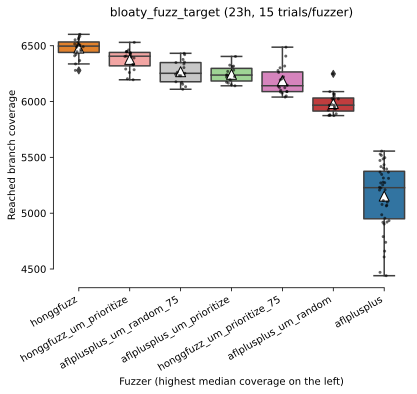
\includegraphics[width=0.75\columnwidth]{bloaty_fuzz_target_boxplot.pdf}
  \caption{AFLplusplus with and without (random) mutant fuzzing: final branch coverage}
  \label{fig:bloatybox}
  
\end{figure}

\begin{figure}
  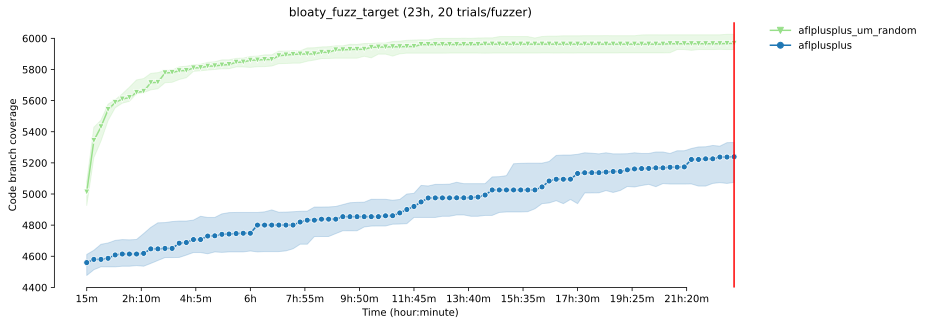
\includegraphics[width=0.75\columnwidth]{bloaty_fuzz_target_coverage_growth.pdf}
  \caption{AFLplusplus with and without (random) mutant fuzzing: branch coverage growth}
  \label{fig:bloatygrowth}  
  \end{figure}

  Figures \ref{fig:bloatybox} and \ref{fig:bloatygrowth} show that in some cases the impact of analyzing mutants can be a very large improvement in code coverage.  In these graphs, directly generated by FuzzBench, {\tt aflplusplus\_um\_random} indicates fuzzing using randomly chosen mutants (um here stands for ``universalmutator'').
Bloaty (\url{https://github.com/google/bloaty}) is not a toy program; like all FuzzBench benchmarks, it is a real-world program, in this case with nearly 4,000 GitHub stars, and over 7,700 lines of code.  Baseline AFLplusplus weak performance shows that it is not an easy target to fuzz effectively.

\begin{figure}
  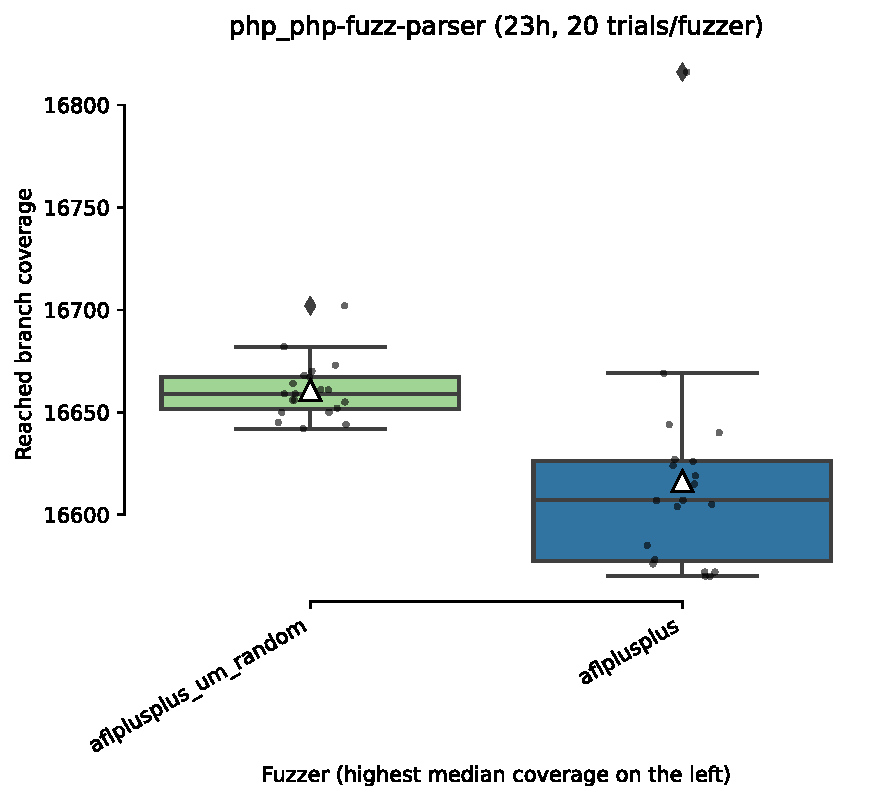
\includegraphics[width=0.75\columnwidth]{php_php-fuzz-parser_boxplot.pdf}
  \caption{AFLplusplus with and without (random) mutant fuzzing: final branch coverage}
  \label{fig:phpbox}
  
\end{figure}

\begin{figure}
  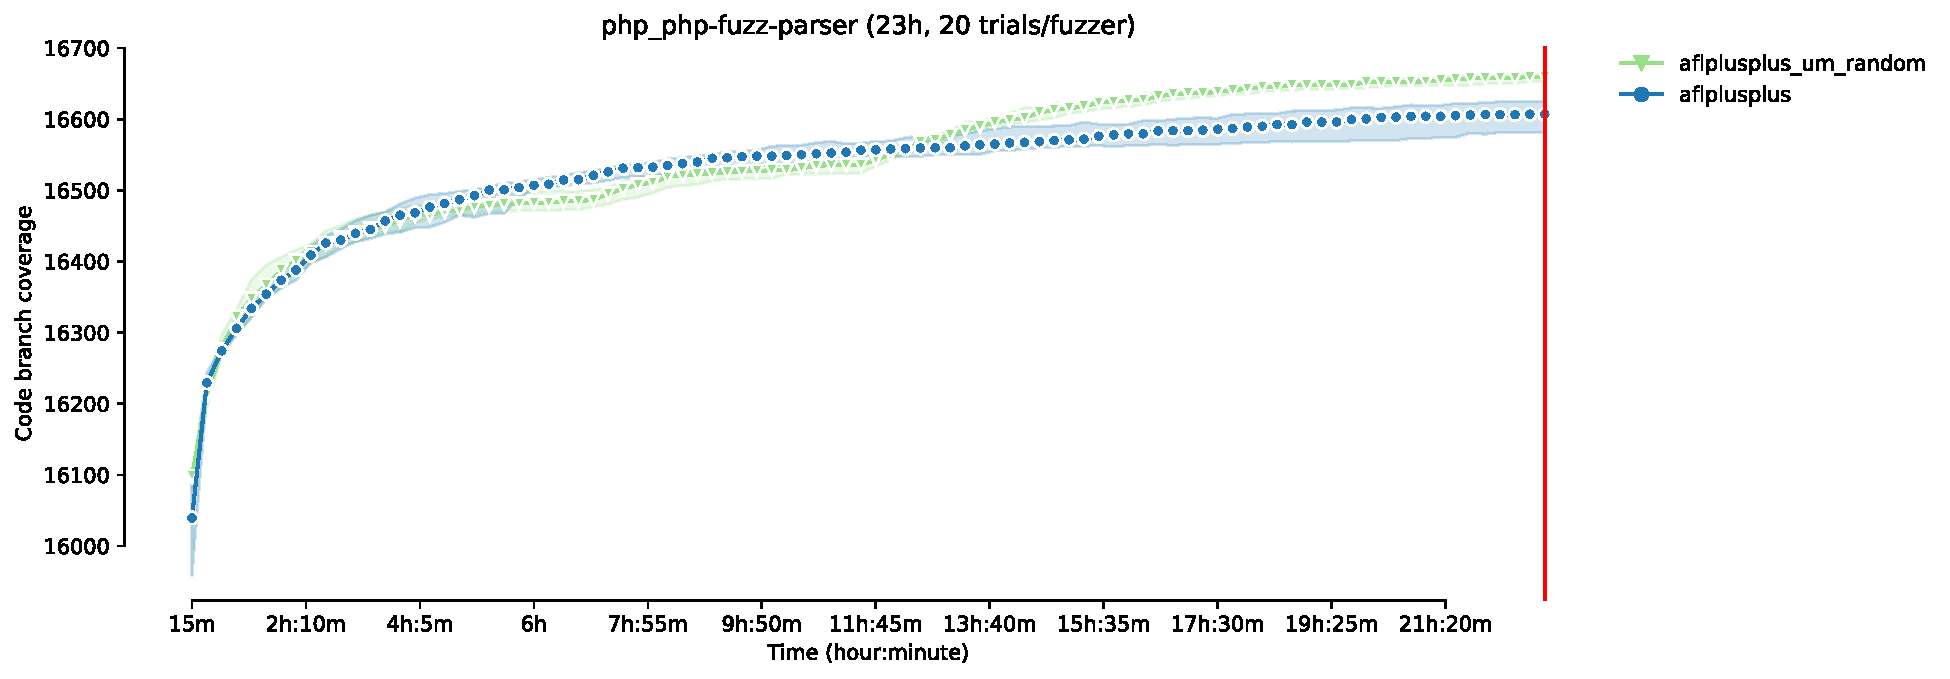
\includegraphics[width=0.75\columnwidth]{php_php-fuzz-parser_coverage_growth.pdf}
  \caption{AFLplusplus with and without (random) mutant fuzzing: branch coverage growth}
  \label{fig:phpgrowth}  
\end{figure}

Figures \ref{fig:phpbox} and \ref{fig:phpgrowth} show that the impact of mutant fuzzing is not always evident during the mutant-fuzzing phase.  Here, the (consistent) advantage over AFLplusplus only appears after fuzzing has swiched to the original target program.  Presumably, seeds generated by some mutants ``pay off'' during the final run of original-target fuzzing.  We note that here and with the bloaty benchmrk, many mutants seem to be essentially equivalent in their impact on fuzzing, since the confidence intervals on branch coverage are tight despite the use of randomly selected, likely non-overlapping mutants.

\begin{figure}
  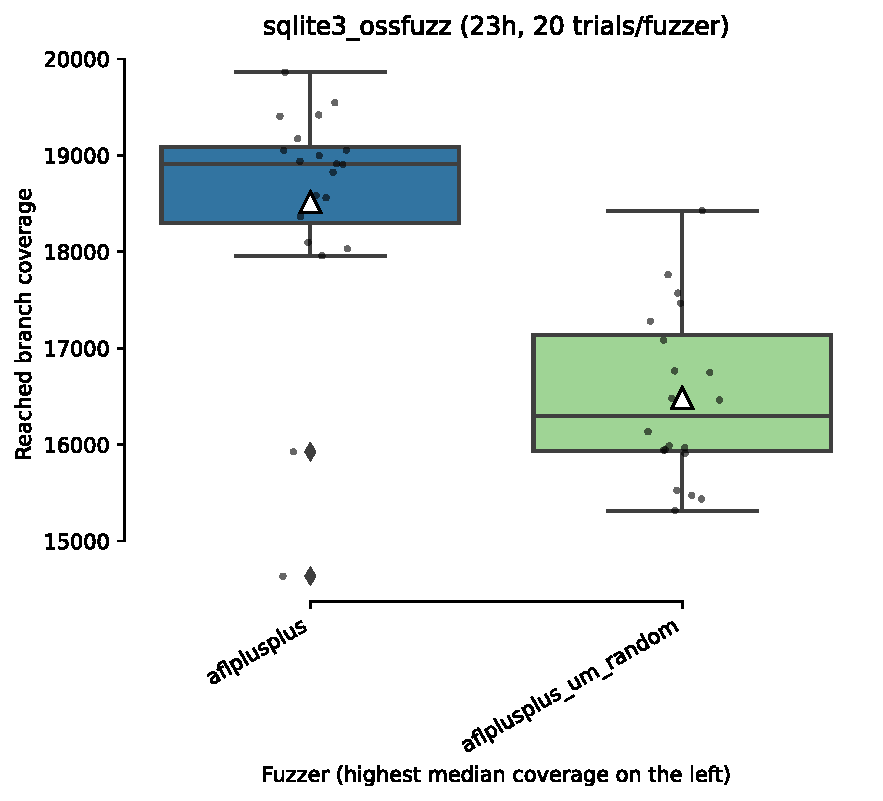
\includegraphics[width=0.75\columnwidth]{sqlite3_ossfuzz_boxplot.pdf}
  \caption{AFLplusplus with and without (random) mutant fuzzing: final branch coverage}
  \label{fig:sqlitebox}
  
\end{figure}

\begin{figure}
  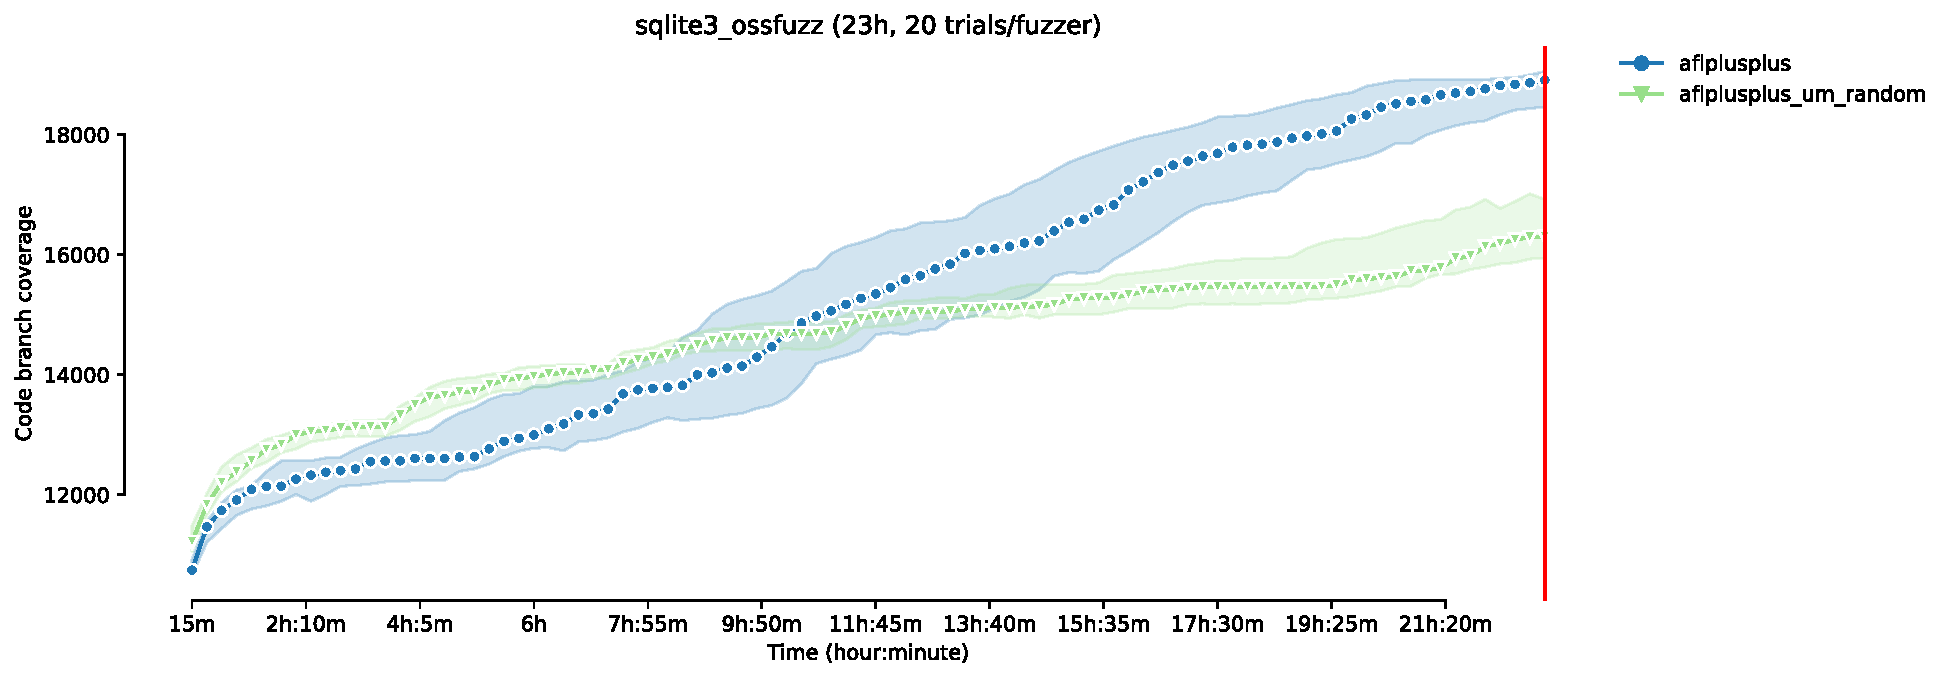
\includegraphics[width=0.75\columnwidth]{sqlite3_ossfuzz_coverage_growth.pdf}
  \caption{AFLplusplus with and without (random) mutant fuzzing: branch coverage growth}
  \label{fig:sqlitegrowth}  
\end{figure}

Finally, it is not always the case that mutants having a strong impact on fuzzing pays off in the long run.  Figures \ref{fig:sqlitebox} and \ref{fig:sqlitegrowth} show that fuzzing mutants can provide a statistically significant advantage over a baseline fuzzer early in the run, but eventually ends up performing significantly worse over a longer period.  We are not sure what causes such results: one possibility is that many mutants are harmful, and the useful mutants that cause the early advantage help with overcoming fuzzing barriers that also can be defeated simply by using a good fuzzer for a longer period.

 \subsection{RQ2: Effects of Mutant Prioritization}

In all cases, the prioritized variants of the approach scored better than using randomly chosen mutants, using the core FuzzBench measures.  In this sense, our results suggest that even a simple prioritization designed for human use is also effective for fuzzing purposes.  On the other hand, comparing individual benchmark median branch coverages, there are ten cases where we have both prioritized and random results for a benchmark, for both AFLplusplus and Honggfuzz.  For AFLplusplus, prioritization is better in three cases, and random mutants are better in three cases.  For Honggfuzz, prioritization is better in seven cases, and random is better in only two cases (however one of these is a very large improvement, from 79.22\% coverage to 91.09\% coverage).

\subsection{RQ3: Non-Cumulative vs. Cumulative Approaches}

Unfortunately, we were unable to run any experiments using the non-cumulative approach.  We discuss the reasons for this omission in detail below.

\subsection{RQ4: Effects of Varying Mutant-Fuzzing Budget}

We would need more fuzzers and more budget allocations to make any claims (and at minimum data for an AFLplusplus prioritized longer mutant phase).  By both FuzzBench measures, AFLplusplus random mutants were improved by running longer, but for Honggfuzz, using 75\%  of the time for mutants was worse for both prioritized and random methods, by both standard FuzzBench measures.  Looking at individual benchmarks, sometimes using mutants longer was helpful, and sometimes it was harmful, but we do note that it seems the changes were not as large as when adding mutants to a fuzzer in general, or changing whether prioritization was used.

\subsection{The FuzzBench Experience}
\label{sec:fuzzexp}

Overall, our experience confirms that FuzzBench is an important contribution to fuzzing research.  The experiments are conducted based on established best practices for fuzzing evaluation \cite{evalfuzz}.  Because of the large number of complex benchmarks included, differences in fuzzers can be demonstrated using only coverage, a metric that is not perfect \cite{FuzzAppeal} but that is also likely to be much more reliable than most bug-count based results on real-world subjects \cite{FuzzAppeal,PLDI13}.  In addition to the kinds of best practices proposed in Klees et al., FuzzBench reports include sophisticated statistical analysis, in order to help researchers report their results honestly.  These go beyond normative software engineering statistical methods \cite{arcuri2014hitchhiker} and include methods from evaluation of machine learning algorithms \cite{CompClass} that are good fits for fuzzing research.  We found the FuzzBench team, especially Jonathan Metz, extremely helpful, and for the most part the development of our experiment code was made easy by the FuzzBench infrastructure.

However, as the incomplete results above show, FuzzBench is not yet an ideal platform for fuzzing research.  In particular, the FuzzBench model made a few assumptions that resulted in great difficulties for us:

\begin{enumerate}
\item FuzzBench assumes it is reasonable to split the experiment into a \emph{build} stage that produces binaries for benchmarks and a \emph{fuzzing} stage that simply consumes binaries.
\item FuzzBench further assumes that \emph{one} build stage per benchmark/fuzzer pair is all that is required.
\item FuzzBench's approach to making the build code for a fuzzer (which may need to, e.g., swap in a new C/C++ compiler) benchmark-agnostic imposes a high cost for builds: each build of a binary builds the entire benchmark, including potentially a large amount of dependency code that needs to be instrumented, from scratch.  For many projects this takes time measured not in seconds but in minutes.
\end{enumerate}

For most fuzzers, where the requirements for the fuzzing stage are one or at most two binaries per benchmark, this works well.  However, because the process prevents us from building binaries for mutants during fuzzing (there is no support for this, and if it were made possible, the need to build completely from scratch for even tiny changes to one file would be unrealistically expensive), and we require hundreds of binaries, our experiments stressed the FuzzBench infrastructure in ways it had not previously been stressed.  Jonathan Metz commented, near the deadline for this submission, ``anyway, y0ur paper did a great job exposing some soft places in fuzzbench's design. I just hope we can handle these before the deadline.''  Among other issues exposed, disk space and limits on debugging logs (to find build issues), plus the problem of pre-emptive cloud instances causing many restarts for experiments with long build times, all introduced long delays in obtaining experimental results or determining why experiments did not run as expected.  Even after the FuzzBench team and ourselves spent over a month (8/25/22 - 10/15/22) debugging our build scripts to work around issues, and in a few cases Jonathan modified FuzzBench parameters or code, some runs and builds failed, and the turnaround for experiments was many times the normal FuzzBench wait.

Due to these issues, our results do not include:

\begin{itemize}
\item {\bf A bug-based evaluation}:  This requires significant time investment including manual labor by the FuzzBench team, after an experiment is complete, and our experiments only finished at the moment of the deadline.  We expect to have such results by publication date, but for a large-scale experiment such as this, the exact timeline is hard to predict.
\item {\bf All desired configurations for mutant-based fuzzing} in particular, the non-cumulative approach, which requires more disk space, is not included.  Exhaustion of disk space during build or fuzz stages was a continual problem for our experiments, so we were advised to not include this approach until those issues can be better resolved.  We also did not extensively experiment with different choices for how much of the fuzzing budget to devote to mutants ({\bf RQ4}); the only variation included is one where 75\%, rather than the default 50\%, of the budget is devoted to mutants.  Similarly, our investigation of {\bf RQ2} is limited to exploring the one prioritization defined by the universal mutator.
\item {\bf All desired fuzzer baselines}: we only compared against AFLplusplus and Honggfuzz.  These are consistently among the  best fuzzers in FuzzBench results, and are both widely used in industry and academia.  However, we would very much like to also examine, at minimum, Eclipser, libFuzzer, and other well-known fuzzers, to see how much the usefulness of our approach varies by benchmark vs. by fuzzer.
  \item {\bf FuzzBench based data for RQ5}: it may be possible to record information to examine {\bf RQ5} in FuzzBench, but we were unable to attempt this due to the problems discussed above; moreover, the time spent getting \emph{any} useful results for the core research question of effectiveness prohibited us from debugging experiments that attempted to answer this question using LAVA-M benchmarks.   We therefore only report RQ5 results for our preliminary experiments.
\end{itemize}

Beyond these omissions, one of our final set of five experiments (combined into a single report with a single coverage normalization) did not actually run, due to as yet undiagnosed build issues
We expect to have results for at least some of these omissions in the near future, but cannot guarantee this for the first two items, since these require efforts by the FuzzBench team beyond simply running additional experiments for us.

It is important to note that \emph{none of these problems are an inherent part of our approach}.  Normally, mutant binaries would be generated on the fly during fuzzing; using incremental builds after modifying a single source line in one file, such changes would usually require a very small part of the fuzzing budget.  This is how our preliminary results were produced, and how the scripts we plan to release for a standalone tool implementing our method work.  Unfortunately, FuzzBench by its nature precludes the fuzzing stage from seeing benchmark source, and forces us to use a cumbersome process that breaks various FuzzBench assumptions.

We further note that the way FuzzBench assembles source files for benchmarks meant that we often ended up mutating code that was not an important part of the benchmark target, but was part of a dependency that was compiled with instrumentation.  In practice, in real world applications, a user would provide a list of relevant source files, which might also limit mutation to critical functionality (e.g., avoiding mutating logging code or user interface code not relevant to a fuzzing harness).

Finally, despite these problems, we encourage other researchers to use FuzzBench in their evaluations!  The primary source of our difficulties, that most fuzzers only use one target binary while we expect to produce and use hundreds or even thousands of binaries, means that \emph{most researchers will not face the challenges we faced.}  On the other hand, FuzzBench introduces a degree of standardization to fuzzing comparisons and, as discussed below, mitigates important threats to validity.  The readability and thoroughness of FuzzBench reports, moreover, made it possible to write up our conclusions, including quality graphics and statistical analyses, in less than a day once final results were available.  Finally, we note that efforts to improve FuzzBench (e.g., the impacts our experiments have had and will have to build infrastructure choices) are available to all researchers, rather than being lost as each team essentially re-invents the wheel.

\section{RQ5: Useful Mutant Types}

Because we were unable to inspect FuzzBench individual mutant impacts, or get LAVA-M based experiments (chosen for direct comparison with T-Fuzz reported results) running in time, due to the difficulty of getting core FuzzBench results, we do not have extensive results to report for this question.  However, we were able to examine the results in preliminary experiments in detail, and see which individual mutants and mutant types contributed most to detecting fuzzgoat bugs not found by at least one of the 10 hour AFL runs.  That is, we looked at cases where the five-minute fuzzing of a mutant found a crash signature that did not appear in at least one of the full AFL runs.  We scored mutants according to how often they contributed to such ``novel bug discovery'' and our findings were suggestive:

\begin{itemize}
\item Overall, only two types of mutant were unusually common among ``bug-finding'' mutants: changing {\tt if} conditionals to false (i.e., removing an entire block of code under an {\tt if}), and adding a {\tt break} to a loop (i.e., removing an entire block of code at the end of a loop).  This suggests that \emph{large-scale} code deletions may provide extra utility.  Surprisingly, statement deletions were not present in the ``most useful'' mutant sets at all.  This may relate to observations made during use of code deletion for resource adaptation, where computed reductions tended to involve large chunks of code \cite{sasomin}; perhaps (somewhat unintuitively) larger deletions are likely to remove fuzzer blocks without compromising functionality to such a degree that behavior no longer resembles the original program.
\item On the other hand, these types of mutants accounted for a minority of useful mutants, and the remaining mutants had no obvious pattern, and even included such unlikely changes as replacing a JSON error string with the empty string (which results in a smaller output buffer size, and perhaps faster fuzzing throughput, is our only speculation as to its utility).
\end{itemize}

Obviously, results over larger and more realistic benchmarks and for full experiments are needed to make strong claims, but it is at least not clear that any particular types of mutants could be safely omitted from the mutation process, given the unusual ways in which mutants contributed to finding rare fuzzgoat bugs.

\section{Comparison with T-Fuzz}

\label{sec:tfuzzfail}

Unfortunately, we were unable to compare our approach with T-Fuzz \cite{tfuzz}.  We attempted to contact the authors, and did contact the author of a more recent fork of the T-Fuzz code, Yoshiki Takashima, who directed us to contact Maverick Woo, who might be able to shed more light on running T-Fuzz.  Both confirmed that they had been unable to get T-Fuzz to run properly after attempting to do so.

We also explored using a Docker image for T-Fuzz (\url{https://hub.docker.com/r/zjuchenyuan/tfuzz}) that contained numerous comments on the original experiments, including some notes on problems with those experiments, developed by the authors of T-Fuzz.  Unfortunately, all T-Fuzz benchmarks, after about ten minutes of fuzzing, with no results produced, terminated with the following form of error message:

{\scriptsize
\begin{code}
  Traceback (most recent call last):
  File "./TFuzz", line 64, in <module>
    main()
  File "./TFuzz", line 55, in main
    tfuzzsys.run()
  File "/T-Fuzz/tfuzz/tfuzz\_sys.py", line 204, in run
    shutil.copyfile(self.fuzzing\_program.program\_path, transformed\_program\_path)
  File "/usr/lib/python2.7/shutil.py", line 69, in copyfile
    raise Error("`\%s` and `\%s` are the same file" \% (src, dst))
shutil.Error: `/T-Fuzz/workdir\_uniq/uniq\_5/uniq` and `/T-Fuzz/workdir\_uniq/uniq\_5/uniq` are the same file
\end{code}
}

Substantial inspection of the source code and further investigation did not result in any way to work around this error, and notes on the Docker suggested that recreating the original experiments might be difficult.  Our failure to duplicate T-Fuzz results (or run T-Fuzz at all) does demonstrate a key difference between our approach and that of T-Fuzz:  while conceptually similar, at a certain level, our approach relies on reliable off-the-shelf components (existing fuzzers and mutation testing tools) and can be implemented in a small script with hooks for fuzzing and target mutation/build.  T-Fuzz, on the other hand, relies on a large number of non-robust components and is clearly subject to ``bit rot'' in fairly short order.

\section{Threats to Validity}

The primary threat to validity here is that our experiments are incomplete.  For some research questions, this essentially makes our results at present not useful.  For the primary research question, {\bf RQ1}, however, there seems to be little doubt, assuming the fuzzer evaluation best-practices encapsulated in FuzzBench are reasonable, that our approach has an overall significant positive effect on branch coverage.  The major threat to validity is that this large advantage in some cases in branch coverage may not translate to an advantage in bug detection.  However, this seems unlikely.  Previous FuzzBench experiments have generally shown a very good correlation between bug and coverage based evaluations.  For example, consider the two reports \url{https://fuzzbench.com/reports/2022-04-19-bug/index.html} and \url{https://fuzzbench.com/reports/2022-04-19/index.html}.  These are coverage and bug-based evaluations for the same set of fuzzers and benchmarks on the same date.  There is some difference in exact rankings, but the overall winners (Honggfuzz and AFLplusplus) are unchanged, and most individual fuzzer pairings are also unchanged.

Some threats to validity present in many fuzzing experiments are likely less relevant to our results:  implementation bugs in the evaluation framework in particular are much less likely, due to the developer support and effort expended by Google on FuzzBench, as well as the probability that any major bugs would be detected over the course of the large number of consequential fuzzer evaluations performed using FuzzBench.






\section{Conclusions and Future Work}

In this paper we propose that by fuzzing variations of a target program generated by a mutation testing tool, it may be possible to work around some fundamental limitations of coverage-driven fuzzing.  For the most part, even when not effective, the technique proposed should be low-cost and at worst equivalent to fuzzing the target program itself for a somewhat smaller time.  Our preliminary experiments show that fuzzing mutants is trivial to implement (and applies to any fuzzer of which we are aware) and effective for improving fault detection, at least for a non-trivial benchmark target program.

Future work, in addition to the performance of full experiments to evaluate the technique, would include exploring the effectiveness of using mutation selection methods and prioritization techniques in addition to those proposed here, and applying directed greybox fuzzing \cite{AFLGo} to specifically target mutated code.  Another possibility is to use Higher Order Mutants \cite{HOM} to fuzz multiple mutants at once; however, this increases the chance that a critical mutant will be combined with a mutant that essentially destroys the program semantics, making it impossible to exploit.


\bibliographystyle{ACM-Reference-Format}

\bibliography{bibliography}

\end{document}
\endinput
%%
%% End of file `sample-manuscript.tex'.
